%%%%%%%%%%%%%%%%%%%%%%%%%%%%%%%%%%%%%%%%%%%%%%%%%%%%%%%%%%%%%%%%%%
\section{Verification of the structural solver}
\label{sec:cantilever}
%%%%%%%%%%%%%%%%%%%%%%%%%%%%%%%%%%%%%%%%%%%%%%%%%%%%%%%%%%%%%%%%%%

\noindent
The three coupled cases that follow all involve a beam undergoing large rotations under a distributed hydrodynamic load, so the beam solver is first exercised in isolation on the static large-deflection cantilever of \citet{belendez_numerical_2003}, subsequently used by \citet{chen_eulerianlagrangian_2019} to validate the structural model of their flexible-vegetation framework. The case suits a combined verification and validation exercise, since the first reference provides experimental tip deflections and the second reports predictions from an independent structural model on the same loading programme.

\noindent
The beam is a slender rectangular-section steel cantilever of length $0.4~\mathrm{m}$, width $25~\mathrm{mm}$ and height $0.4~\mathrm{mm}$, giving $EI = 0.02591~\mathrm{N\,m^2}$ with $E = 194.3~\mathrm{GPa}$ and $G = 74.73~\mathrm{GPa}$. The height-to-length ratio of $10^{-3}$ places it in the large-deformation regime even at moderate loads, and at the largest load the free end displaces vertically by approximately $70\%$ of the beam length, which makes a linearised analysis inapplicable. The beam carries a uniformly distributed self-weight of $0.758~\mathrm{N\,m^{-1}}$ together with a vertical concentrated load at the free end, varied from $0$ to $0.588~\mathrm{N}$. It is solved on a uniform discretisation of $80$ beam cells with a fully clamped root and a free tip, advanced in pseudo-time to a static steady state.

\noindent
Table~\ref{tab:cantilever} reports the free-end vertical displacement and Figure~\ref{fig:cantilever_load_deflection} shows the load--deflection curve together with the deformed centrelines. The incremental stiffness decreases progressively as the beam rotates away from its initial configuration and the moment arm of the applied load shortens, which the geometrically exact formulation captures without linearisation of the kinematic relationships. The maximum difference from the experimental measurements is $1.74\%$, at $F = 0.098~\mathrm{N}$, and all other cases remain at or below $0.93\%$. The elevated error at the smallest nonzero load reflects the proximity of that case to the self-weight-dominated equilibrium, where the concentrated load contributes only modestly above the self-weight effect and the percentage difference is correspondingly sensitive to small discrepancies in the applied load or material parameters. At every other load the difference stays below $1\%$ without a systematic trend, the two largest cases giving $0.78\%$ and $0.93\%$. Against the independent structural model, the two agree to four decimal places in metres at every load level except $F = 0.294~\mathrm{N}$, where the present prediction of $0.2270~\mathrm{m}$ lands on the experimental measurement while the reference value differs by $0.09\%$. The structural solver is therefore both validated against the measurements and verified against an independent model before it is embedded in the coupled cases.

\begin{table}[!ht]
\centering
\small
\caption{Large-deflection cantilever benchmark. Free-end vertical displacement $\delta_y$ under applied tip load $F$, comparing the experimental measurements of \citet{belendez_numerical_2003}, the values reported by \citet{chen_eulerianlagrangian_2019}, and the present finite volume beam solver.}
\label{tab:cantilever}
\setlength{\tabcolsep}{4pt}
\renewcommand{\arraystretch}{1.1}
\begin{tabularx}{\linewidth}{c c >{\centering\arraybackslash}X c c c}
\toprule
& \multicolumn{3}{c}{Free-end vertical displacement $\delta_y$ (m)} & \multicolumn{2}{c}{Difference vs.\ experiment (\%)} \\
\cmidrule(lr){2-4}\cmidrule(lr){5-6}
$F$ (N) & Experiment & Chen and Zou (structural model) & This work & Chen and Zou & This work \\
\midrule
0.000 & 0.089 & 0.0898 & 0.0898 & 0.90 & 0.90 \\
0.098 & 0.149 & 0.1516 & 0.1516 & 1.74 & 1.74 \\
0.196 & 0.195 & 0.1960 & 0.1960 & 0.51 & 0.51 \\
0.294 & 0.227 & 0.2272 & 0.2270 & 0.09 & 0.00 \\
0.392 & 0.251 & 0.2495 & 0.2495 & 0.60 & 0.60 \\
0.490 & 0.268 & 0.2659 & 0.2659 & 0.78 & 0.78 \\
0.588 & 0.281 & 0.2784 & 0.2784 & 0.93 & 0.93 \\
\bottomrule
\end{tabularx}
\end{table}

\begin{figure}[!ht]
\centering
\begin{subfigure}[b]{0.49\textwidth}
  \centering
  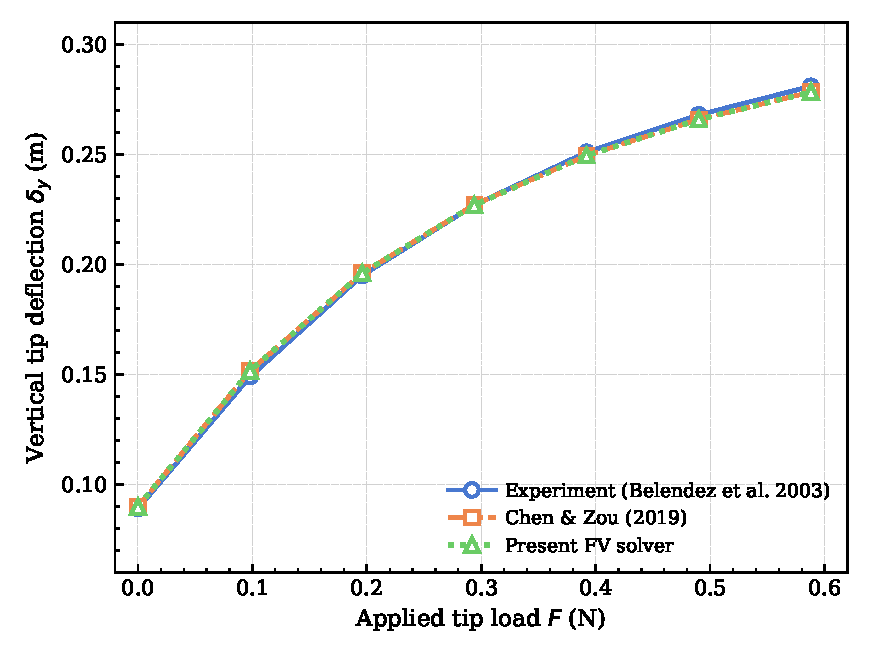
\includegraphics[width=\linewidth]{cantilever_load_deflection.pdf}
  \caption{}
\end{subfigure}\hfill
\begin{subfigure}[b]{0.49\textwidth}
  \centering
  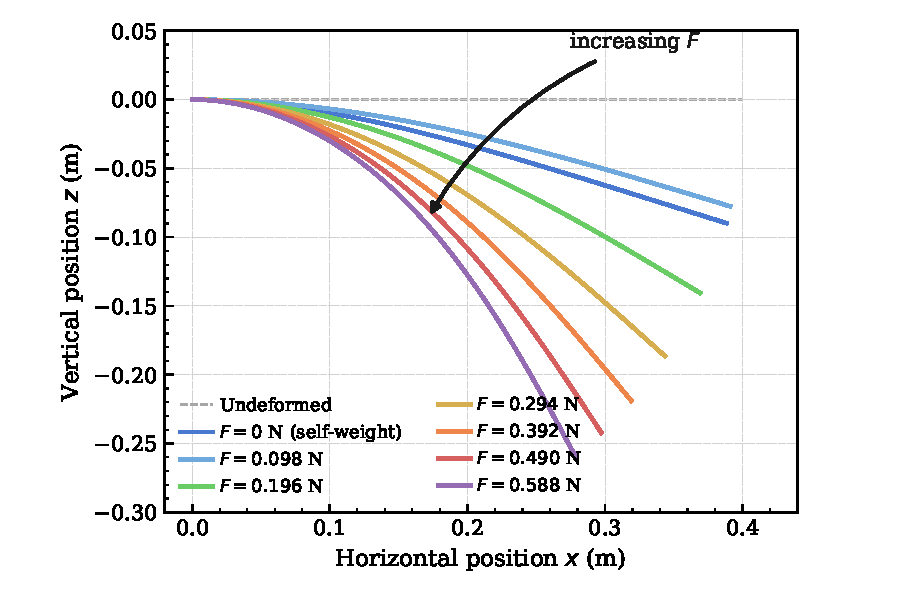
\includegraphics[width=\linewidth]{largeDeflectionCantileverLoads.pdf}
  \caption{}
\end{subfigure}
\caption{Large-deflection cantilever benchmark. (a) Load--deflection curve, comparing the experimental measurements of \citet{belendez_numerical_2003}, the structural model of \citet{chen_eulerianlagrangian_2019}, and the present finite volume Simo--Reissner beam solver. (b) Deformed centrelines predicted by the present solver under self-weight and increasing vertical end load.}
\label{fig:cantilever_load_deflection}
\end{figure}

